\documentclass{article}
\usepackage[utf8]{inputenc}

\usepackage{titlesec}
\newcommand{\sectionbreak}{\clearpage}

\title{Documentation \\ \textbf{AutonomousDJ} \\ CIR}

\author{Benedikt Novotny, Florian König, Tim Wieschalla}
\date{January 2018}

\usepackage{natbib}
\usepackage{graphicx}
\usepackage{color}

\begin{document}

\maketitle

\tableofcontents


% ==============================================================================
% ==============================================================================
\section{Introduction}


The robot presented in this report is intended to replace a human DJ at indoor parties. Like a professional DJ it should be able to select and play the preferred music of the crowd and get people to dance. It should do so by learning from the reaction of the people to the played music up until now.

\begin{figure}[ht!]
\centering
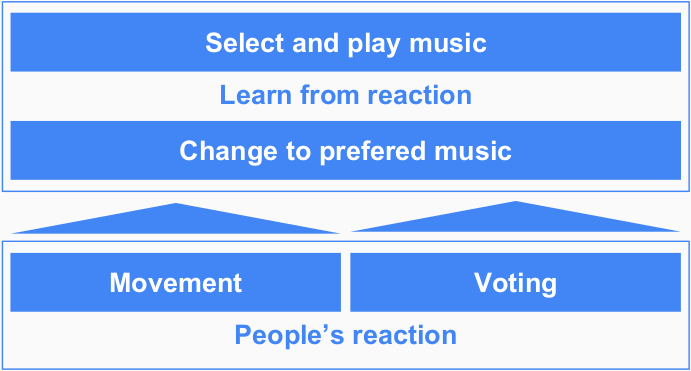
\includegraphics[scale=0.5]{Idea.png}
\caption{Main Idea}
\label{fig:idea}
\end{figure}


% ==============================================================================
% ==============================================================================
\section{Interaction Aspects}


% ==============================================================================
%\subsection{Storyboard}

\begin{figure}[ht!]
\centering
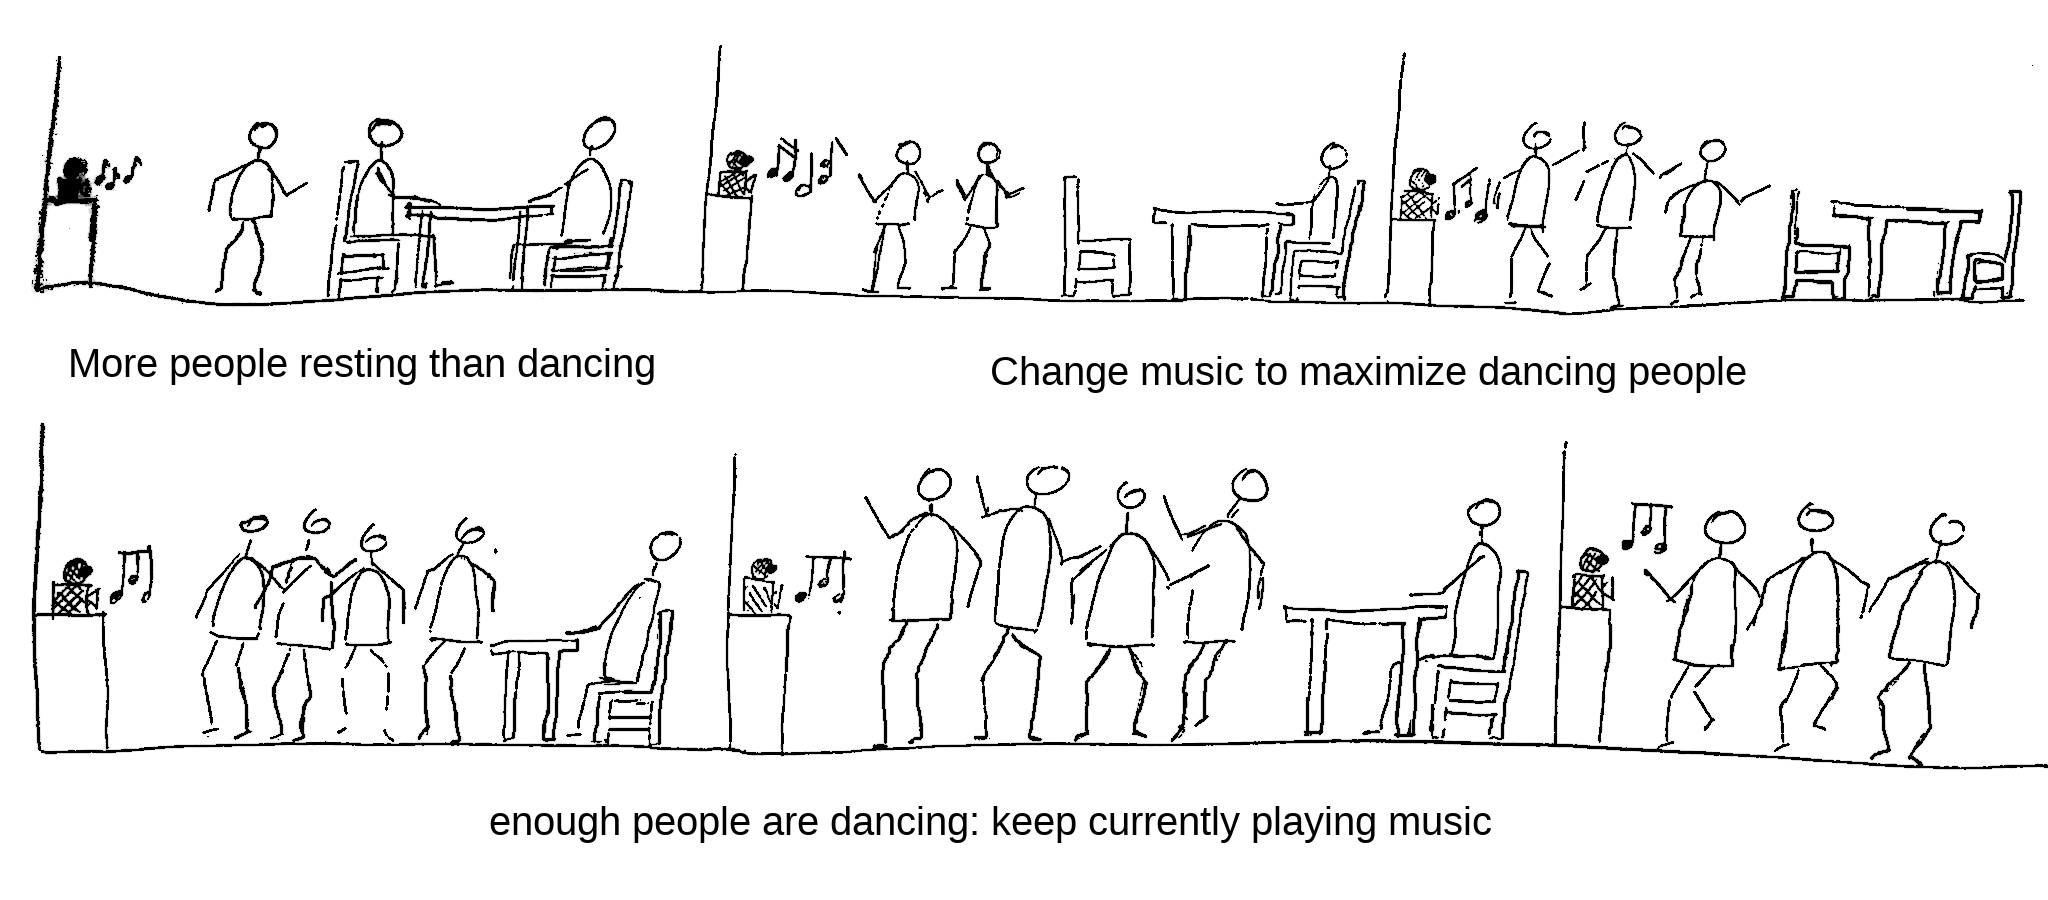
\includegraphics[scale=0.15]{storyboard.png}
\caption{Storyboard}
\label{fig:functionalities}
\end{figure}

% =============================================================================
\subsection{Purpose and Application Field}

The role of this robot is to be an autonomous DJ with the capabilities of choosing and playing music on its own. Its purpose is to get as many people to dance as possible. \\
The application field of the robot would be indoor parties where the hiring of a professional DJ would not be cost effective but the host does not want to take care of the music selection her/himself.

The role of our robot is an autonomous DJ which is able to learn about the peoples music taste and can analyze whether the people like the currently played song or not. To be able to act in his role the robot needs a number of functionalities. The main functionalities can be split in two parts as shown in Figure 1: Changing the music on the one hand and receiving the peoples music taste by using different sensor data in a learning process. The two parts will be closer explained in the following sections.

% =============================================================================
\subsection{Appearance}

It was intended to build a custom body for the robot. Approximately the size of a shoe box that could sit on an elevated surface like a table or dresser. It would have included a webcam, speakers and a simple light indicator in traffic light style. This idea was given up as it was problematic to prepare a RaspberryPi computer with all the libraries needed to run the already written software. Instead the software is able to run on an ordinary laptop that already has all the hardware features needed.

% =============================================================================
\subsection{Competences and Skills}

To achieve this goals the robot needs to be able to perceive the impact of the played music on the people. To this end it should be able to measure the amount of dancing people via picture analysis of the webcam stream. This proved to be a relatively hard problem to solve. In the course of the development we settled for the option of measuring the density of people on the dancefloor.\\
To help the learning process and steer it faster in the right direction we further implemented a webservice were people could vote on the currently playing song (like / dislike it). \\
The robot takes the perceived and given information on the mood of the crowd and displays its finding in a simple traffic light style manner (red, yellow, green) and of course tries to steer the changing of the music into the 'green' zone.

% =============================================================================
\subsection{Detailed Requirement Analysis}

\subsubsection{Context}
\begin{itemize}
    \item Physical Scenario\\
Indoor room with a dancing space

\item Social Environment\\
    Adults in a relaxed environment

\item Role\\
    To entertain the people through music and motivate them to dance

\item Functions\\
    Playing music, signaling the perceived mood in the room

\item Tasks\\
    Change the music to maximize the people dancing

\end{itemize}

\subsubsection{Target User Profile}
\begin{itemize}
\item Age\\
    Adults and young adults

\item Genre\\
    No specific genre of people

\item Preferences\\
    Adults who enjoy dancing

\item Capabilities / Impairments\\
    People should bring the capability to dance
    No specific focus on any impairments.
\end{itemize}

\subsubsection{Platform}
\begin{itemize}
\item Technical Description\\
    The robot will be a non moving entity approximately the size of a shoebox and will sit on a dresser or table. Alternatively a Notebook can fulfill the same function.

\item Robots social features
\begin{itemize}
    \item Appearance\\
        A robot without any humanoid features. Appears more like a simple stereo or common Laptop.
    
    \item Social Affordances\\
        Natural like or bioinspired features: None
        Non-natured features: No special discernible features

    \item Communicative Skills and Interactive Behaviour\\
        Verbal: None
        Non verbal: Playing music, Simple color signaling, Web-Interface
\end{itemize}
\end{itemize}

\subsubsection{Performance}
\begin{itemize}
    \item Behaviour\\
        Plays music, indicates perceived mood
    \item Social behaviour\\
	    Tries to guess the mood in the room by analysing the amount of movement in the picture. \\
	    Consider manual Feedback through Webinterface.\\
	    Learn musical preferences of the crowd.\\
	    Changes music according to perceived mood and already learned preferences.\\
\end{itemize}

% =============================================================================
\subsection{Additional Research: Interview with a DJ}
The interview was carried out and recorded in German. The following is the summarized and translated transcription of the recorded interview. The DJ we talked to works for many types of events but mostly on weddings. Due to this he decided to refer his answers to a wedding like setting and not a club setting. The DJ could confirm some of our previous approaches. Furthermore, he provided additional and new insights in the decision making of a human DJ. \\
\\
\textbf{Which songs do you use to start?}\\
I refer to a wedding like setting now. In clubs it is different. I usually start with two or three chart songs that everyone knows, and everyone knows the lyrics of. \\
\\
\textbf{When should a genre change be performed?}\\
Approximately three songs of one genre, then a slow change.\\
\\
\textbf{Do you sometimes try to guess the music taste?}\\
Yes of course, it depends for example on the age distribution in the group. \\
\\
\textbf{How do you decide which song will be played next? How extreme can changes be?} \\
The transitions should be as soft as possible. But later, when wished songs are played, extreme changes are possible. And then the speed of the sing, the rhythm and the BPM – beats per minute – of two songs following each other should fit together. And I have many transitions that worked before which I always play. For example, “Play it alive” from Safri Duo and a Latin-American version of “Marathon” form Helene Fischer. \\
\\
\textbf{Which are the indicators whether the crowd likes the music or not?} \\
For example, if the sitting people are moving their feeds or people are singing the played song these are good indicators that they like the song. To test it, you can mute the song for a moment and check whether the people continue singing. Furthermore, the number of people who are entering or leaving the dance floor is a good indicator. And then you just notice. \\
\\
\textbf{When should a song change be performed?} \\
A good point for a song change is, when there is only a bass line without voice. That is a good point for a transition. Possible is also to change at the end of a sentence or at points where a change would be logical regarding the lyrics. \\
\\
\textbf{Should songs always be played until the end} \\
At the beginning, there should be more transitions between songs. The end can be skipped to play more different songs. Later, when wished songs are played, the songs can or should be played until the end.  

% =============================================================================
\subsection{Abandoned Ideas}

\textbf{Noise level analysis}\\
Happy dancing people do not only move on the dancefloor but also vocalize their joy. A microphone could be used to measure the simple noise level. However as at the same time music is played in the room it would be difficult the filter out the played music to only get the noise level of the people.


% ==============================================================================
% ==============================================================================
\section{Technical Aspects}


% ==============================================================================
\subsection{Hardware}

The original plan was to use a RaspberryPi and construct an own body around it - including a webcam and speakers. Due to the space restrictions on the storage space we had on the RaspberryPi we were not able to compile needed libraries. Instead the software was to run on a Laptop in the end.

% ==============================================================================
\subsection{Operating System: Linux}

The most common OS for the RaspberryPi would be the Raspian Linux Distribution. It is a derivative of Debian that is customized especially for the RaspberryPi and comes with the same huge software repository. \\
For developing on non-linux OSes we used VirtualBox to emulate Debian.

% ==============================================================================
\subsection{Programming Language: Python}

Python is fast to develop and available for multiple operating systems. It would make it easier to later port the software to other soft- and hardware platforms. \\
Python is also popular among developers in general and comes with great support and documentation. It runs on Linux and comes with bindings for the OpenCV library.

% ==============================================================================
\subsection{Video processing: Open CV}

OpenCV is a free computer vision library that comes with many functionalities that are interesting for analysing the video stream:
\begin{itemize}
    \item Person detection
    \item Face recognition
    \item Emotion detection
    \item ...
\end{itemize}
Although OpenCV can be used to detect and count persons in videos it does fail to do so when the persons are not clearly separated. So this option is not useful for counting people in a dancing crowd. \\
We then used an edge detection algorithm (Canny Edge Detection - also provided by the OpenCV library) to reduce noise in the video stream. This gave us frames that could be compared more easily to each other.\\
The final approach was first to let the user tune the parameters of the edge detection to the environment (lighting is always a factor) and capture an empty frame that is later used to compare all following frames. A simple pixel-by-pixel comparison of the (possibly) crowded dancefloor against the first empty frame should give a good approximation of the density of people dancing.\\

% ==============================================================================
\subsection{Spotify API}

To play and choose music the Spotify API was chosen. The Spotify API has several advantages: 
\begin{itemize}
    \item Offers song recommendations from simple parameters
    \item Huge library of music already available
    \item Music already classified in several parameters
\end{itemize}
The API offers 14 parameters that can be given to the recommendation functionality additionally to the genre. 126 genres are available and we chose 33 suitable for dancing. From the parameters we chose 3:
\begin{itemize}
    \item Energy\\
        A float-value between 0 and 1 that expresses the perceived energy conveyed by the song
    \item Tempo\\
        Beats per minute of the song
    \item Valence\\
        A float-value between 0 and 1 that expresses the perceived positiveness of the song.
\end{itemize}
All in all that gives us 4 parameters that can be changed in combination with the q-learning algorithm to let the API choose the next for us. \\
Not only is it possible to choose songs with the API but it also is possible to create, manipulate and control the playback of playlists with the API - the only thing that is needed is a running spotify client (it can be running independently on any other device) to let the music play.

% ==============================================================================
\subsection{Q-Learning}

-blabla
-idea: graph implemented as table.
-vertices define the songs, genre and bpm
-edges between them show the success of the songs after they were played
-initalized by 0


[Text]

\begin{figure}[ht!]
\centering
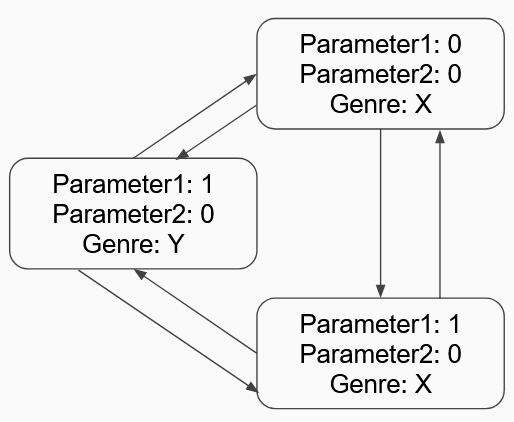
\includegraphics[scale=0.5]{QLearning.png}
\caption{Q-Learning}
\label{fig:q-learning}
\end{figure}

% ==============================================================================
\subsection{Implementation}

The implementation is rather straight forward:
\begin{itemize}
    \item Initialize the video stream, choose the parameters for the edge detection and capture a frame of the empty dance floor.
    \item Initialize Spotify API - a spotify account is needed that has to permit our software access to it for creating playlists and changing the playback.
    \item Start the Webservice for manual feedback
    \item Initialize an empty Q-Learning algorithm
    \item Loop:
    \begin{itemize}
        \item Get parameters from Q-Learning to feed to the Spotify API to retrieve a song recommendation
        \item Add the song to the playlist and start playback
        \item Wait for the song to finish and gather the mood of the crowd via webcam and webservice
        \item Feed the perceived mood to the Q-Learning
        \item Reset the manual submitted votes to 0
    \end{itemize}
\end{itemize}



% ==============================================================================
% ==============================================================================
\section{Evaluation}


During our own testing we already noticed that the q-learning is converging too slowly to the preferred music. In the early stages 

Possible question for participants:\\
- How did you like the music that the autodj chose?\\
- Did it inspire you to dance?\\
- Do you think it improved over time?\\
- Did you like/use the possibility of manual feedback?\\
- Would you use the autodj for your own party?\\
- What would you improve?


% ==============================================================================
% ==============================================================================
\section{Future Work}


\begin{itemize}
    \item Build custom body\\
        Find an image for RaspberryPi where all neccessary libraries are already compile. \\
        Design and construct a body around the RaspberryPi to unclude a Webcam and simple LEDs.
    
    \item Improve mood and crowd detection\\
        There are more techniques to process the video stream. More research probably will lead to a better result.\\
        Noise detection could also be implement to get a better idea of mood of the crowd.
    
    \item Improve learning system \\
        Provide pre-set models that do not learn everything from the ground up and maybe already center around a certain genre.\\
        Refine parameters of the Q-Learning-Model.
    
    \item Improve the manual Feedback\\
        The design and functionality of the webservice at this point is most basic. It is questionable if dancing people will interact with it at all. A more reasonable perspective is to implement it in a way to only dislike the currently playing song. Only dissatisfied people will take the time to cast a vote. 
\end{itemize}


% ==============================================================================
% ==============================================================================
% \section{Conclusion}

% \citep{adams1995hitchhiker}

\bibliographystyle{plain}
\bibliography{references}
\end{document}
